\documentclass{BHCexam}
%\usepackage[colorlinks,linkcolor=black]{hyperref}
\begin{document}
\biaoti{极坐标和参数方程}
\fubiaoti{}
\maketitle
\tableofcontents
\section{极坐标}
\subsection{极坐标的定义}
在平面内取一个定点$ O $ ,叫做极点,自极点$ O $引一条射线$ Ox $,叫做极轴;再选定一个长度单位,一个角度单位(通常取弧度)及其正方向(通常取逆时针方向),这样就建立了一个极坐标系.如下图:
\begin{center}
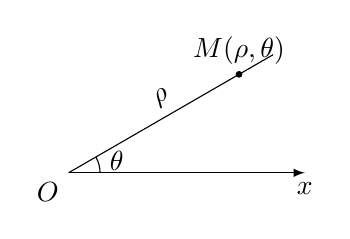
\begin{tikzpicture}
\coordinate [label=below left:$O$](O) at(0,0);
\draw[->,>=latex] (O)--(3,0) node[below] (x) {$x$};
\draw (O)--(30:3) node[midway,sloped,above] (p){$\rho$};
\node[above] (M)at(30:2.5){$M(\rho,\theta)$};
\draw[fill] (30:2.5) circle (1pt);
\draw (0.4,0) arc (0:30:0.4);
\node[right] (t)at (0.4,0.15) {$\theta$};
\end{tikzpicture}
\end{center}
{\kaishu
极坐标系四要素:\ding{192}极点;\quad \ding{193} 极轴;\quad \ding{194}长度单位;\quad \ding{195} 角度单位和正方向.}\par 
点$M$的极坐标:设$ M $是平面内一点,极点$ O $与点$ M $的距离$ \abs{OM} $叫做点$ M $的极径,记为$ \rho $;以极轴 为始边,射线$ OM $为终边的$ M $叫做点$ M $的极角,记为$ \theta $.有序数对$ (\rho,\theta) $叫做点$ M $的极坐标,记为$ M(\rho,\theta) $. \par
{\kaishu 注:\ding{192}极坐标$ (\rho,\theta) $与$ (\rho,\theta+2k\pi)(k\inZ) $表示同一个点。极点$ O $的坐标为$ (0,\theta)(\theta\inR) $;\par
\ding{193}一般的,不做特殊说明情况下,$ \rho\ge0 $.}
\subsection{极坐标与直角坐标的互化}
\noindent 互化的前提条件:
\begin{enumerate}[1)]
\item 极坐标系中的极点与直角坐标系中的原点重合;
\item 极轴与$x$轴的正半轴重合;
\item 两种坐标系中取相同的长度单位.
\end{enumerate}
\begin{center}
\begin{tikzpicture}
\coordinate [label=below left:$O$](O) at(0,0);
\draw[->,>=latex] (O)--(3,0) node[below] (x) {$x$};
\draw[->,>=latex] (O)--(0,3) node[right] (y) {$y$};
\draw (O)--(30:2.5) node[midway,sloped,above] (p){$\rho$};
\node[above] (M)at(30:2.5){$M(\rho,\theta)$};
\draw[fill] (30:2.5) circle (1pt);
\draw (0.4,0) arc (0:30:0.4);
\node[right] (t)at (0.4,0.15) {$\theta$};
\coordinate (m) at ($(O)!(30:2.5)!(3,0)$);
\coordinate(d) at($(O)!(30:2.5)!(0,3)$);
\draw (30:2.5)--(d) node[midway,above]{$x$};
\draw(30:2.5)--(m)node[midway,right]{$y$};

\end{tikzpicture}
\end{center}
\noindent 互化公式:
$$\Bigg\{\begin{aligned}
x=\rho \sin \theta\\x=\rho \cos \theta
\end{aligned}$$ 或者$$\Bigg\{\begin{aligned}
&\rho ^2=x^2+y^2\\&\tan \theta =\dfrac{y}{x}(x\ne0)
\end{aligned}$$
\subsection{常用极坐标方程}
\begin{enumerate}[1)]
\item 直线的极坐标方程:若直线过点$ M(\rho_0,\theta_0) $,且极轴到此直线的角为$\alpha$,则它的方程为:$$\rho\sin(\theta-\alpha)=\rho_0\sin(\theta_0-\alpha)$$特别的:
\begin{enumerate}[a)]
\item 当直线$ l $过极点,即$ \rho_0=0 $时,直线$ l $的极坐标方程为$ \theta=\alpha (\rho\inR)$或写成:$\theta=\alpha $及$ \theta=\alpha+\pi $;
\item 直线过点$ M(a,0) $且垂直于极轴时,直线$ l $的极坐标方程为:$\rho\cos \theta=a$;
\item 直线过$ M(a,\dfrac{\pi}{2}) $且平行于极轴时,直线$ l $的极坐标方程为:$ \rho\sin\theta=b $;
\end{enumerate}
\item 圆的极坐标方程: 若圆心为$ M(\rho_0,\theta_0) $,半径为$r$的圆方程为:$$\rho^2-2\rho_0\rho\cos(\theta-\theta_0)+\rho_0^2-r^2=0$$特别的:
\begin{enumerate}[a)]
\item 圆心在极轴上点$ (a,0) (a>0)$处,且圆过极点$ O $的圆的方程:$\rho=2a\cos\theta$;
\item 圆心在极轴上点$ (a,\dfrac{\pi}{2}) (a>0)$处,且圆过极点$ O $的圆的方程:$\rho=2a\sin\theta$;
\end{enumerate}
\end{enumerate}
注意事项:
\begin{enumerate}[1)]
\item 极坐标与直角坐标可以相互转化,但是不能直接相互调用化简(参数方程可以直接代入到直角坐标方程中);
\item 求解极坐标方程有关问题,主要有两种方法:
\begin{enumerate}[(1)]
\item 直接解极坐标方程,联立极坐标方程得到$ \theta $和$ \rho $,这种方法在解曲线交点时比较方便;
\item 将极坐标方程转化为直角坐标方程,用直角坐标方程进行求解,这种方法可以避免方程理解错误,但是有些时候计算不是很方便.
\end{enumerate}
\end{enumerate}
\subsection{练习}
\begin{questions}

\qs 在极坐标系中,圆$ \rho=-2\sin \theta $的圆心的极坐标方程是\xx
\onech{$ \left(1,\dfrac{\pi}{2}\right)$}{$ \left(1,-\dfrac{\pi}{2}\right)$}{$ \left(1,0\right)$}{$ \left(1,\pi\right)$}
\qs 在极坐标系中,曲线$\rho=2\cos\theta $是\xx
\twoch{过极点的直线}{半径为$ 2 $的圆}{关于极点对称的图形}{关于极轴对称的图形}
\qs 极坐标方程$ \left(\rho-1 \right)\left(\theta-\pi\right)=0\left(\rho\ge0\right) $表示的图形是\xx
\twoch{两个圆}{两条直线}{一个圆和一条射线}{一条直线和一条射线}
\qs 在极坐标系中,曲线$ \rho=4\sin\left(\theta-\dfrac{\pi}{3}\right) $关于\xx
\fourch{直线$\theta=\dfrac{\pi}{3} $轴对称}{直线$\theta=\dfrac{\pi}{6} $轴对}{点$\left(2,\dfrac{\pi}{3}\right) $对称}{极点中心对称}
\qs 若以直角坐标系的原点为极点,$x$轴的非负半轴为极轴建立极坐标系,则线段$ y=1-x (0\le x\le 1)$的极坐标为\xx
\fourch{$ \rho=\dfrac{1}{\cos\theta+\sin\theta},0\le \theta\le\dfrac{\pi}{2}$}{$\rho=\dfrac{1}{\cos\theta+\sin\theta},0\le \theta\le\dfrac{\pi}{4} $}{$\rho=\cos\theta+\sin\theta,0\le \theta\le\dfrac{\pi}{2} $}{$ \rho=\cos\theta+\sin\theta,0\le \theta\le\dfrac{\pi}{4}$}
\qs 在极坐标系中,点$ \left(2,\dfrac{\pi}{6}\right) $到直线$ \rho\sin\theta =2$的距离等于\tk.
\qs 在极坐标系中,直线$ \rho\cos\theta-\sqrt{3}\rho\sin\theta-1=0 $与圆$ \rho=2\cos\theta $交于$ A,B $两点,则$ \abs{AB}= $\tk.
\qs 在极坐标系中,点$ \left(2,\dfrac{\pi}{3}\right) $到直线$ \rho\left(\cos\theta+\sqrt{3}\sin\theta\right)=6 $的距离为\tk.
\qs 在极坐标系中,点$ A $在圆$ \rho^2-2\rho\cos\theta -4\rho\sin\theta+4=0$上,点$ P $的坐标为$ (1,0) $,则$ \abs{AP} $的最小值为\tk.
\qs 在平面直角坐标系$xOy$中,曲线$ C_1:\Bigg\{\begin{aligned}
x=t\cos \alpha\\
y=t\sin\alpha.
\end{aligned}(t\text{为参数},t\ne0) $其中$ 0\le\alpha\le\pi $,在以$ O $为极点,$x$轴正半轴为极轴的极坐标系中,曲线$ C_2:\rho=2\sin\theta ,~C_3:\rho=2\sqrt{3}\cos\theta$.
\begin{parts}
\part 求$ C_1 $与$ C_3 $交点的直角坐标;
\part 若$ C_1 $与$ C_2 $相交于点$ A,~  C_1 $与$ C_3 $相交于点$ B $,求$ \abs{AB} $的最大值.
\end{parts}


\end{questions}




\newpage
\section{参数方程}
\subsection{参数方程的概念}
在平面直角坐标系中,若曲线$C$上的点$ P(x,y) $满足$\Bigg\{\begin{aligned}
x=f(t),\\y=g(t).
\end{aligned}$该方程叫曲线C的参数方程,变量t是参变数,简称参数.{\kaishu
(在平面直角坐标系中,如果曲线上任意一点的坐标 都是某个变数 的函数 $\Bigg\{\begin{aligned}
x=f(t),\\y=g(t).
\end{aligned}$并且对于$ t $的每一个允许值,由这个方程所确定的点$ M(x,y) $都在这条曲线上,那么这个方程就叫做这条曲线的参数方程,联系变数$ x,y $的变数$ t $叫做参变数,简称参数.)}
\subsection{常用参数方程}
\begin{enumerate}
\item 直线的参数方程:\[\Bigg\{\begin{aligned}
&x=x_0+t\cos \alpha\\
&y=y_0+t\sin\alpha 
\end{aligned}{~(t\text{为参数})}
\]
\begin{center}
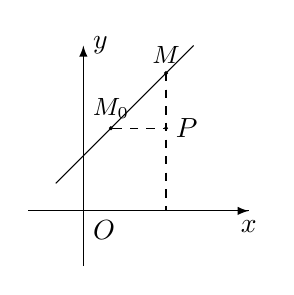
\begin{tikzpicture}[scale=0.7]
\coordinate[label=below right:$O$] (O) at(0,0);
\coordinate[label=below:$x$] (x) at(3,0);
\coordinate[label=right:$y$] (y) at(0,3);
\draw[->,>=latex](-1,0)--(x);
\draw[->,>=latex](0,-1)--(y);
\draw[domain=-0.5:2] plot(\x,{\x +1});
\coordinate[label=above :\small$M_0$](M0) at(0.5,1.5);
\coordinate[label=above:\small $M$](M) at(1.5,2.5);
\draw[fill] (M) circle (0.7pt);
\draw[fill] (M0) circle (0.7pt);
\draw[dashed](M)|-(M0);
\draw[dashed] (M)|-(x);
\coordinate[label=right:$P$](P) at(1.5,1.5);
\draw[fill] (P) circle (0.7pt);
\end{tikzpicture}
\end{center}
{\kaishu $(x_0,y_0)$为直线上定点$ M_0 $的坐标,$ (x,y) $为直线上任意一点$ M $的坐标,$ \alpha $为倾斜角,$ t $为$ \abs{MM_0} $长度,若$M_0$所对应的参数为$ t_1 $,$ M $所对应的参数为$ t_2 $,则有$ \abs{MM_0}=\abs{t_2-t_1} $.}
\item 圆的参数方程:\[\Bigg\{\begin{aligned}
&x=x_0+R\cos\theta \\
&y=y_0+R\sin\theta
\end{aligned}~(\theta\text{为参数})\]{\kaishu 其中$\theta \in\left[0,2\pi\right)$,圆心为$ M_0(x_0,y_0) $,半径为$ R(R\ge0),M(x,u) $为圆上任意一点.}
\item 椭圆的参数方程:
\[\Bigg\{\begin{aligned}
&x=a\cos\varphi\\
&y=b\sin\varphi
\end{aligned}(\varphi\text{为参数})\]
{\kaishu 其中$\varphi\in\left[0,2\pi\right)$,注意$ \varphi $不是椭圆上的点和原点连线的夹角,是椭圆对应的圆的离心角.}
\item 双曲线的参数方程:\[\Bigg\{\begin{aligned}
x=a\sec\theta\\
y=b\tan \theta
\end{aligned}
{~(\theta\text{为参数})}\]
\item 抛物线$ y^2=2px $的参数方程可表示为:\[\Bigg\{\begin{aligned}
&x=2pt^2\\&y=2pt
\end{aligned}(t\text{为参数})\] 
\end{enumerate}
\subsection{练习}
\begin{questions}

\qs 曲线$\Bigg\{\begin{aligned}
&x=-1+\cos\theta\\
&y=2+\sin\theta.
\end{aligned}(\theta\text{为参数})$的对称中心\xx
\twoch{在直线$y=2x $上}{在直线$y=-2x $上}{在直线$y=x-1 $上}{在直线$y=x+1 $上}
\qs  圆$\Bigg\{\begin{aligned}
x=-1+\sqrt{2}\cos\theta,\\
y=1+\sqrt{2}\sin\theta 
\end{aligned}(\theta\text{为参数})$被直线$ y=0 $截得的劣弧长为\xx
\onech{$ \dfrac{\sqrt{2}\pi}{2}$}{$ \pi$}{$ 2\sqrt{2}\pi$}{$ 4\pi$}
\qs 已知曲线$ C:\Bigg\{\begin{aligned}
&x=\dfrac{\sqrt{2}}{2}t\\
&y=a+\dfrac{\sqrt{2}}{2}t
\end{aligned} (t\text{为参数}),A(-1,0),B(1,0).$若曲线$ C $上存在点$ P $满足$ \vv{AP}\bm{\cdot}\vv{BP}=0 ,$则实数$ a $的取值范围是\xx
\onech{$ \left[-\dfrac{\sqrt{2}}{2},\dfrac{\sqrt{2}}{2}\right]$}{$ \left[-1,1\right]$}{$ \left[-\sqrt{2},\sqrt{2}\right]$}{$ \left[-2,2\right]$}
\qs 点$ P(1,0) $到曲线$\Bigg\{\begin{aligned}
&x=t^2,\\
&y=2t
\end{aligned}~(\text{其中参数}t\inR$)上的点的最短距离是\xx
\onech{$ 0$}{$ 1$}{$ \sqrt{2}$}{$ 2$}
\qs 曲线$\Bigg\{\begin{aligned}
&x=\cos\theta\\
&y=1+\sin\theta 
\end{aligned}(\theta \text{为参数})$与直线$ x+y-1=0 $相交于$ A,B $两点,则$ \abs{AB}= $\tk.
\qs 曲线$ C:\Bigg\{\begin{aligned}
&x=\cos\theta\\
&y=-1+\sin\theta.
\end{aligned}(\theta\text{为参数}) $的普通方程是\tk;如果曲线$ C $与直线$ x+y+a=0 $有公共点,那么实数$ a $的取值范围是\tk.
\qs 已知动点$ P,Q $都在曲线$ C:\Bigg\{\begin{aligned}
&x=2\cos t,\\
&y=2\sin t.
\end{aligned} (t\text{为参数})$上,对应参数分别为$ t=\alpha $与 $ t=2\alpha(0<\alpha<2\pi) $,$ M $为$ PQ $的中点.
\begin{parts}
\part 求$ M $的轨迹的参数方程;
\part 将$ M $到坐标原点的距离$ d $表示为$ \alpha $的函数,并判断$ M $的轨迹是否过坐标原点.
\end{parts}
\kongbai
\qs 已知曲线$C_1$的参数方程是$\Bigg\{\begin{aligned}
&x=2\cos\varphi,\\
&y=3\sin\varphi.
\end{aligned}(\varphi\text{为参数})$,以坐标原点为极点,$x$轴的正半轴为极轴建立极坐标系,曲线$C_2$的极坐标方程是$\rho=2$.正方形$ABCD$的顶点都在$C_2$上,且$A,B,C,D$以逆时针次序排列,点$A$的极坐标为$(2,\dfrac{\pi}{3})$.
\begin{parts}
\part 求点$ A,B,C,D $的直角坐标;
\part 设点$ P $为$ C_1 $上任意一点,求$ \abs{PA}^2+\abs{PB}^2+\abs{PC}^2+\abs{PD}^2 $的取值范围.
\end{parts}
\kongbai 
\qs 已知曲线$ C:\dfrac{x^2}{4}+\dfrac{y^2}{9}=1 $,直线 $\Bigg\{\begin{aligned}
&x=2+t\\
&y=2-2t
\end{aligned}(t\text{为参数}) $.
\begin{parts}
\part 写出曲线$ C $的参数方程,直线$ l $的普通方程;
\part 过曲线$ C $上任意一点$ P $作与直线$ l $夹角为$ 30^{\circ} $的直线,交$ l $于点$ A. $求$ \abs{PA} $的最大值与最小值.
\end{parts}
\kongbai
\qs 在直角坐标系中$ xOy $中,曲线$ C_1 $的参数方程为$\Bigg\{\begin{aligned}
&x=2\cos\alpha\\
&y=2+2\sin\alpha
\end{aligned}(\alpha\text{为参数})$,$ M $是$ C_1 $上的动点,$ P $点满足$ \vv{OP}=2\vv{OM} $,$ P $点的轨迹为曲线$ C_2 $.
\begin{parts}
\part 求$ C_2 $的方程;
\part 在以$ O $为极点,$x$轴正半轴为极轴的极坐标系中,射线$ \theta=\dfrac{\pi}{3} $与$ C_1 $的异于极点的交点为$ A $,与$ C_2 $的异于极点的交点为$ B $,求$ \abs{AB} $.
\end{parts}
\end{questions}
\end{document}